$$
\begin{aligned}
&\oiint_{\Sigma} \vec{B}\cdot\hat{n}dS = 0 \qquad\ \ \forall \ \Sigma \text{ chiusa di } \mathbb{R}^3\\
&\oint_\Gamma \vec{M}\cdot\hat{t}dl = i_{\Gamma\text{ lib}} \qquad \forall \ \Gamma \text{ chiusa di } \mathbb{R}^3\\
&\vec{B} = \mu_0(\vec{H} + \vec{M}) \\
&[H] = [M] = \si{\ampere\per\meter} \\
& \vec{M} = \mathcal{M}[\vec{H}] \qquad\qquad \text{Relazioni costitutive}
\end{aligned}
\qquad
\begin{aligned}
&\oiint_\Sigma \vec{D}\cdot\hat{n} dS = Q_{\text{lib}} \ \qquad \forall \ \Sigma \\
&\oint_\Gamma\vec{E}\cdot\hat{t} dl = 0 \ \qquad\qquad\ \forall \ \Gamma \\
&\vec{D} = \varepsilon_0\vec{E} + \vec{P}\\
&[D] = [P] = \si{\coulomb\per\meter^2}\\
&\vec{P} =\mathcal{P}[\vec{E}]
\end{aligned}
$$

Le relazioni costitutive nei dielettrici possono essere lineari ad es. $\vec{P} = \varepsilon_0\chi_e\vec{E} $

Si richiamano ora invece le equazioni di Maxwell in condizioni non stazionarie.
$$
\begin{aligned}
&\oiint_\Sigma \vec{B}\cdot\hat{n} dS = 0 \qquad\qquad\qquad\qquad\qquad \forall\ \Sigma\\
&\oint_\Gamma \vec{H}\cdot\hat{t}dl = i_{\Gamma \text{ lib}} + \iint_{S_\Gamma} \frac{\partial \vec{D}}{\partial t} \cdot\hat{n} dS\qquad \forall \ \Gamma\\
&\vec{B} = \mu_0(\vec{H} + \vec{M}) \\
& \vec{M} = \mathcal{M}[\vec{H}] 
\end{aligned}
\qquad
\begin{aligned}
&\oiint_\Sigma \vec{D}\cdot\hat{n}dS = Q_{\text{lib}_{\Omega_\Sigma}}\\
&\oint_\Gamma \vec{E}\cdot\hat{t}dl = -\iint_{S_\Gamma} \frac{\partial\vec{B}}{\partial t}\cdot\hat{n}dS\\
&\vec{D} = \varepsilon_0\vec{E} + \vec{P}\\
&\vec{P} =\mathcal{P}[\vec{E}]
\end{aligned}
$$
Conservazione della carica
$$
\oiint_\Sigma \vec{J}_{\text{lib}}\cdot\hat{n}dS = - \iiint_{\Omega_\Sigma}\frac{\partial \rho_\text{lib}}{\partial t} dV \qquad \forall \Sigma
$$

\subsection{Relazioni costitutive dei materiali magnetici}
È necessario comprendere l'azione di un campo $\vec{B}$ su una spira di raggio $r$ percorsa da corrente $i$
\begin{figure}[H]
\centering
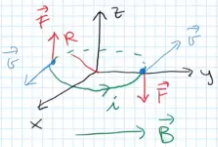
\includegraphics[width = 0.4\linewidth]{forza_lorentz_spira}
\end{figure}
$$
\vec{B} = B_0\ \vec{e}_y
$$
La carica sarà soggetta alla forza di Lorentz, supponendo $\vec{E} = 0$
$$
\vec{F} = q\vec{v}\times\vec{B}
$$
Le due forze sono uguali opposte e se la spira è rigida sarà sottoposta ad una coppia 
di momento
$$
\vec{M}_F = (\vec{r}_{p'}-\vec{r}_{p''}) \times\left(\frac{m_e \vec{v}}{m_e}q\times\vec{B}\right)
$$
Ma il vettore che congiunge i due punti è parallelo a $\vec{B}$ quindi l'equazione 
precedente gode della proprietà associativa del doppio prodotto vettoriale (solitamente non 
valida)
$$
\vec{a}\times(\vec{b}\times\vec{a}) = -(\vec{b}\times\vec{a})\times\vec{a} = (\vec{a}\times
\vec{b})\times\vec{a}
$$
$$
\vec{M}_F = \left[(\vec{r}_{p'}-\vec{r}_{p''})\times m_e\vec{v}\right] \times\frac{q}{m_e}\vec{B}
$$
Il termine tra parentesi quadre è il momento angolare orbitale della particella (elettrone) 
$\vec{L}_e$ mentre $\frac{q}{m_e} = \gamma$ si ottiene
$$
\vec{M}_F = \gamma \vec{L}_e \times\vec{B} = \vec{\mu}\times\vec{B}
$$
Si hanno due posizioni di equilibrio se $\vec{mu}$ e $\vec{B}$ sono parallele, stabile
se sono equiverse. Un momento elementare tende ad allinearsi con il campo $\vec{B}$ esterno.

Gli elettroni possiedono in generale un momento magnetico pari alla somma del momento 
orbitale e del momento magnetico intrinseco (spin) responsabile per il 90\% del 
comportamento magnetico dei materiali.

Si caratterizzano i materiali in base alla loro risposta ad un campo magnetico
esterno:
\begin{itemize}
\item[Apolari] - Non ci sono momenti magnetici in assenza di campo
\item[Polari] - A temperatura ambiente i momenti magnetici elementari sono orientati
casualmente
\end{itemize}

Si consideri una sostanza apolare, sottoposta successivamente ad un campo $\vec{H}$, a 
causa di un effetto chiamato \href{https://it.wikipedia.org/wiki/Precessione_di_Larmor}{Precessione di Larmor} si ha un allineamento degli elettroni antiparallelamente al campo
subendo un effetto chiamato diamagnetico.

Una sostanza polare invece ha un momento magnetico medio nullo dovuto all'orientamento 
casuale dei momenti magnetici molecolari a causa dell'agitazione termica. 
Applicando il campo esterno $\vec{H}$ si vede un momento magnetico diverso da zero
orientato parallelamente al campo $\vec{H}$. Questo fenomeno avviene nei materiali 
paramagnetici.

\begin{figure}[H]
\centering
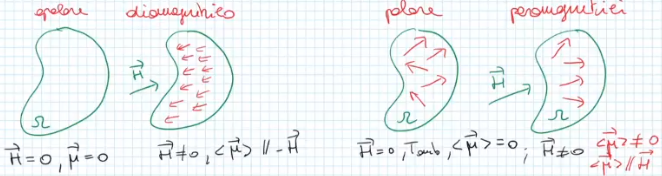
\includegraphics[width = 0.7\linewidth]{diamagneti_paramagneti}
\end{figure}

In entrambi questi tipi di materiali $\vec{M} = \chi_m \vec{H}$ con $\chi_m$ maggiore di 
zero per i paramagnetici e minore di zero per i diamagnetici.
$\chi_m$ è detta suscettività magnetica ed è adimensionale.

Gli ordini di grandezza sono i seguenti:
\begin{align*}
\chi_m = \begin{cases}
-10^{-5} \qquad \text{ diamagentici}\\
10^{-4} \div 10^{-3} \text{ paramagnetici}
\end{cases}
\end{align*}
Di conseguenza per i materiali è possibile introdurre una permeabilità $\mu$ che tenga
in considerazione la suscettività dello stesso
$$
\vec{B} = \mu_0 (\vec{H} + \chi_m\vec{H}) = \mu_0 (1+\chi_m)\vec{H} = \mu\vec{H}
$$
$$
\mu = \mu_0\mu_r \qquad \mu_r = (1-10^{-5},1 + 10^{-3})
$$
Si vede dunque che i materiali diamagnetici e paramagnetici sono poco rilevanti e possono
essere approssimati con il vuoto ($\mu\simeq\mu_0$).

Invece elementi come Fe,Ni,Co e alcune delle loro rispettive leghe sono materiali
ferromagnetici, presentano una magnetizzazione spontanea anche in assenza di un campo su 
scala macroscopica.
Se si suppone di non applicare un campo esterno, un materiale ferromagnetico si presenta
ad un'analisi microscopica ad effetto Kerr, detta \href{https://en.wikipedia.org/wiki/Magneto-optic_Kerr_effect}{MOKE}, una tecnica con la quale si misura la riflessione
di un raggio laser da parte del materiale, proporzionale alla sua magnetizzazione.

Si osserva il materiale come se fosse suddiviso in regioni, denominate \href{https://it.wikipedia.org/wiki/Dominio_di_Weiss}{domini di Weiss}, separate dalle cosiddette
pareti di dominio, in cui i momenti magnetici dei dipolini sono tutti orientati tra loro.

\begin{figure}
\centering
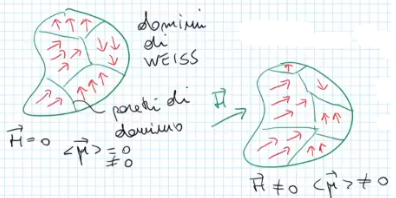
\includegraphics[width = 0.6\linewidth]{materiali_ferromagnetici_weiss}
\end{figure}

Il momento magnetico medio di un simile materiale può essere o meno pari a zero
a seconda di come sono orientati i domini. L'applicazione di un campo esterno tende
a rimpicciolire i domini non orientati concordemente e ingrandire quelli orientati
concordemente mediante un moto delle pareti.

Aumentando sempre di più il modulo del campo esterno, resterà soltanto un dominio orientato
parallelamente al campo esterno, lo spostamento delle pareti permane parzialmente
anche in assenza del campo.

I materiali ferromagnetici esibiscono una dipendenza dello stato di magnetizzazione
attuale dalla storia precedente, fenomeno noto come isteresi magnetica.

\newpage
La configurazione di equilibrio viene stabilita attraverso la competizione di quattro 
interazioni, le prime due di origine microscopica (\textit{short-range}), se esistessero
solo queste si avrebbe un unico dominio allineato con la direzione ``facile''. Le 
interazioni 3 e 4 vengono chiamate \textit{long-range}.
\begin{enumerate}
\item Interazione di scambio, allinea gli spin vicini, è un'interazione di origine quantistica responsabile della formazione dei domini
\item Anisotropia magneto-cristallina, esistono direzioni facili o difficili di magnetizzazione a seconda della forma del reticolo
\item Interazione magnetostatica, una magnetizzazione produce un campo ``di reazione'' 
detto campo demagnetizzante e tende a favorire l'assenza di cariche magnetiche, a causa
di un costo energetico superiore ad una configurazione di spin antiparalleli
\item Interazione con il campo esterno, allineamento degli spin con il campo esterno, 
chiamata anche interazione \href{https://it.wikipedia.org/wiki/Effetto_Zeeman}{Zeeman}
\end{enumerate}
L'equilibrio dei domini è il risultato dell'unione di questi fenomeni. Un fattore cruciale
è la dimensione del corpo, su scale microscopiche l'interazione di scambio è la 
predominante, si avrà un singolo dominio, si avrà frammentazione all'aumentare della scala.

\subsection{Curva di isteresi magnetica}
È possibile misurare l'isteresi scalare se il campo $\vec{B}$ e $\vec{H}$ sono allineati,
oppure se si hanno geometrie particolari come un toro o un provino di \href{https://en.wikipedia.org/wiki/Epstein_frame}{Epstein}. 

Curva di isteresi a seguito di una trasformazione periodica tra due valori di $\vec{H}$
in una trasformazione ``lenta'' trascurando le correnti di spostamento.

Dall'origine degli assi il sistema segue una curva chiamata ``di prima magnetizzazione'',
questa non potrà superare il valore asintotico $M_s$ chiamato magnetizzazione di 
saturazione, punto in cui non ci sono più domini da allineare. Raggiunto il valore $H_{\text{max}}$ si riduce il campo magnetico ma il corpo non seguirà la curva precedente 
ma segue una curva differente che passa per il punto $M_R$ detta 
\textit{magnetizzazione residua} o rimanenza.

Se si applica un campo negativo si raggiunge un campo nel punto $H_C$ detto \textit{campo 
coercitivo}, campo di segno opposto necessario ad annullare la magnetizzazione.

Si raggiunge infine un nuovo asintoto ancora di saturazione, e ritornando indietro
con il campo $\vec{H}$ si ottiene una curva speculare alla precedente.

\begin{figure}[H]
\centering
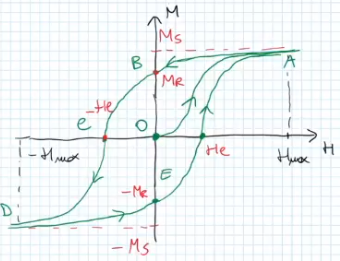
\includegraphics[width = 0.6\linewidth]{ciclo_isteresi_magnetica}
\end{figure}

Se si riduce gradualmente il campo tra un ciclo e l'altro si raggiunge un nuovo ciclo detto
``minor loop'', si vede quindi che per raggiungere un certo punto del piano è necessario
seguire un certo percorso.

I cicli di isteresi sono solitamente simmetrici e vengono suddivisi solitamente
in categorie:
\begin{itemize}
\item Materiali morbidi, hanno un ciclo di isteresi ``stretto'' con alta saturazione e 
basso campo coercitivo, ad esempio Fe-Si, utilizzati principalmente nelle macchine
elettriche. L'area piccola del ciclo di isteresi corrisponde a piccole perdite di energia
\item Materiali duri, hanno un alto campo coercitivo e un'alta saturazione, hanno un ciclo
``largo'' ad esempio NdFeB, SmCo utilizzati nei magneti permanenti o dove serve 
un grande prodotto $H\cdot M$.
\end{itemize}

\subsection{Lavoro eseguito dai generatori in una variazione del campo magnetico}
Preso un toro di materiale ferromagnetico sul quale viene posto un avvolgimento massiccio 
che lo concatena percorso da corrente.
La spira $\Omega_S$ è sede della corrente $\vec{J}_0$ e di un campo elettromotore 
$\vec{E}_m$, ci sarà un campo $\vec{B}$ in tutto lo spazio.

Si suppone di variare il campo
$$
\Delta\vec{B} = \frac{\partial \vec{B}}{\partial t} \Delta t
$$
Utilizzando le eq. di Maxwell in forma locale
$$
\nabla\times\vec{E} = -\frac{\partial \vec{B}}{\partial t} \Rightarrow \nabla\times\vec{E} 
+ \nabla \times \left(\frac{\partial \vec{A}}{\partial t}\right) = 0 \Rightarrow 
$$
$$
\nabla\times\left(\vec{E}+\frac{\partial\vec{A}}{\partial t}\right) = 0
$$
Il campo $\left(\vec{E} + \frac{\partial \vec{A}}{\partial t}\right)$ è conservativo e 
quindi esprimibile come il gradiente di un campo potenziale:
$$
\vec{E} = -\frac{\partial \vec{A}}{\partial t} - \nabla\varphi = -\vec{E}_m
$$
con $\varphi$ potenziale scalare.

I generatori compensano $\vec{E}$ con un campo $\vec{E}_m$ opposto per non far
variare $\vec{J}_0$, la potenza necessaria ad effettuare questa compensazione è pari
a 
$$
P^{(a)}_{\text{gen}} = \iiint_{\Omega_S} \vec{E}_m\cdot\vec{J}_0 dV = 
\iiint_{\Omega_\infty} \left(\frac{\partial \vec{A}}{\partial t} \cdot\ \vec{J}_0 + \nabla\varphi \vec{J}_0\right) dV
$$
Siccome $\vec{J}_0$ sono le correnti sorgenti del campo magnetico allora $\vec{J}_0 = \nabla\times\vec{H}_a$
è dunque un campo solenoidale, moltiplicato per un campo conservativo $\nabla\varphi$.
Vale la seguente identità vettoriale
$$
\nabla\cdot(\varphi \nabla\times \vec{H}_a) = \varphi\cancel{\nabla\cdot(\nabla\times\vec{H}_a)} +
\nabla\varphi\cdot\nabla\times\vec{H}_a
$$
Sostituendo il secondo termine dell'integrale
$$
\iiint_{\Omega_\infty}\nabla\varphi\cdot\nabla\times\vec{H}_a dV = \iiint_{\Omega_\infty} \nabla\cdot(\varphi\nabla\times\vec{H}_a) dV \stackrel{\text{T. Divergenza}}{=} \iint_{\partial\Omega_\infty} \varphi\nabla\times\vec{H}_a\cdot\hat{n}dS = 0
$$
L'integrale è pari a zero per la normalità all'infinito dei campi quindi l'equazione
della potenza fornita dal generatore resta
$$
P^{(a)}_{\text{gen}} =
\iiint_{\Omega_\infty} \left(\frac{\partial \vec{A}}{\partial t} \cdot\ \vec{J}_0 \right) dV = \iiint_{\Omega_\infty} \frac{\partial \vec{A}}{\partial t} \cdot\ \left( \nabla\times\vec{H}_a \right) dV
$$
Ricordando che $\nabla\cdot(\vec{v}\times\vec{w}) = \vec{w}\cdot\nabla\times\vec{v} -  \vec{v}\cdot\nabla\times\vec{w}$, si pone $\vec{w} = \frac{\partial \vec{A}}{\partial t}$ e
$\vec{v} = \vec{H}_a$

Per la normalità all'infinito $\nabla\cdot(\vec{v}\times\vec{w}) = 0$ è quindi possibile
scambiare i termini nel prodotto vettoriale ossia $\vec{w}\cdot\nabla\times\vec{v} = \vec{v}\cdot\nabla\times\vec{w} $, nell'integrale si ha
$$
P^{(a)}_{\text{gen}} = \iiint_{\Omega_\infty} \frac{\partial \vec{A}}{\partial t} \cdot\ \left( \nabla\times\vec{H}_a \right) dV = \iiint_{\Omega_\infty} \vec{H}_a \cdot\ \left( \nabla\times\frac{\partial \vec{A}}{\partial t} \right) dV
$$
Invertendo la derivata temporale con quella spaziale
$$
P^{(a)}_{\text{gen}} = \iiint_{\Omega_\infty}\vec{H}_a \cdot\frac{\partial}{\partial t} \nabla\times\vec{A} dV =  \iiint_{\Omega_\infty}\vec{H}_a \cdot \frac{\partial \vec{B}}{\partial t} dV
$$
Il lavoro svolto dal generatore è pari a 
$$
\Delta L_{\text{gen}} = P^{(a)}_{\text{gen}} \Delta t = \iiint_{\Omega_\infty} \vec{H}_a
\cdot\Delta\vec{B} dV
$$

In una variazione ciclica come quella di isteresi magnetica il lavoro svolto è
$$
\Delta L_{\text{gen}}^{(\text{ciclo})} = \oint_{\text{ciclo}} \iiint_{\Omega_\infty} \vec{H}_a\cdot d\vec{B} dV = \iiint_{\Omega_\infty} \left(\oint_{\text{ciclo}} \vec{H}_a \cdot d\vec{B}\right) dV = <p^{(a)_{\text{mat}}}> T 
$$
Il prodotto tra parentesi è proprio l'area del ciclo di isteresi nel punto $p$, mentre
l'integrale di volume esterno rappresenta la somma delle aree del ciclo in tutti i punti 
dello spazio. La perdita per isteresi è inoltre lineare con la frequenza di alimentazione.
